% Permission is granted to copy, distribute and/or modify this document
% under the terms of the GNU Free Documentation License, Version 1.2
% or any later version published by the Free Software Foundation;
% with no Invariant Sections, no Front-Cover Texts, and no Back-Cover
% Texts.  A copy of the license is included in the section entitled "GNU
% Free Documentation License".
% Copyright 2015 EDF
%

%%%%%%%%%%%%%%%%%%%%%%%%%%%%%%%%%%%%%%%%%%%%%%%%%%%%%%%%%%%%%%%%%%%%%%%%%%%%%%%%%%%%%%%%%%
\section{Architecture guide}

This document makes up the general specification design for the general linear model stepwise regression analysis
in OpenTURNS.

\subsection{LinearModelAlgorithm}

\texttt{LinearModelAlgorithm} derive from \texttt{MetaModelAlgorithm}, with standard pimpl idiom
as prescribed by OpenTURNS coding rules.

\begin{figure}[htb]
  \begin{center}
    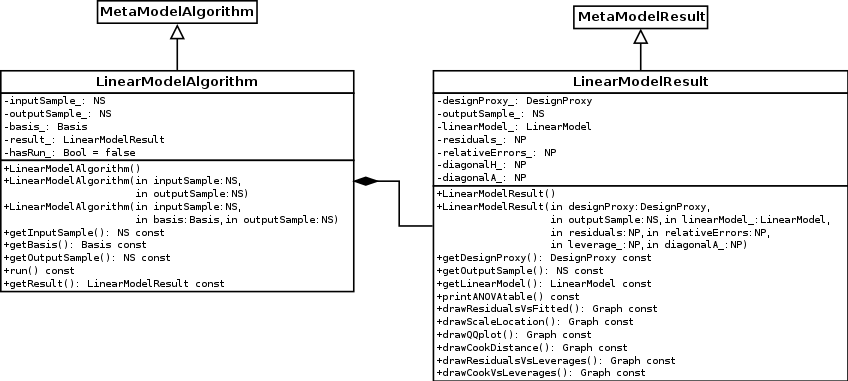
\includegraphics[scale=0.5]{LinearModelAlgorithm.png}
    \caption{LinearModelAlgorithm class}\label{fig:archi:LinearModelAlgorithm}
  \end{center}
\end{figure}

\texttt{LinearModelStepwiseFactory} derive from \texttt{PersistentObject}
\begin{figure}[htb]
  \begin{center}
    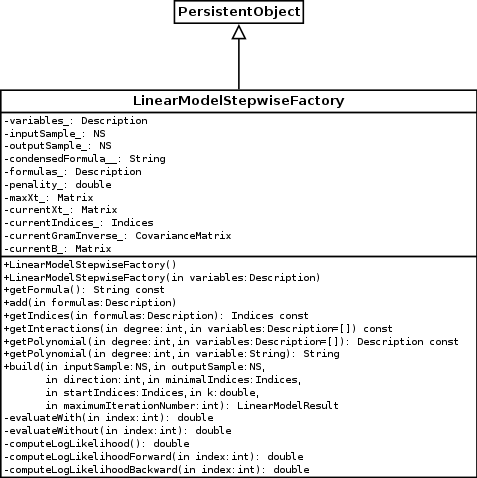
\includegraphics[scale=0.5]{LinearModelStepwiseFactory.png}
    \caption{LinearModelStepwiseFactory class}\label{fig:archi:LinearModelStepwiseFactory}
  \end{center}
\end{figure}
